
\lec{2}{09/02/25}{Intro to Entropy  and Mutual Information}


\begin{defn}{Entropy}{}

  \textit{Entropy} is a measure of the uncertainty of a random variable. Let \(X\) be a discrete random variable with alphabet \(\mathcal{X} \) and probability mass function \(p_{X} (x) = \mathrm{Pr} \left\{ X = x \right\}, \; x \in \mathcal{X}  \). The \textit{entropy} \(H(X)\) of a discrete random variable \(X\) is defined by 
\[
  H(X) =  \sum_{x \in \mathcal{X} } p(x) \log _2 \frac{1}{p(x)} = - \sum_{x \in \mathcal{X} } p(x) \log _2 p(x) = \mathbb{E}_{p}  \left[ \log _2 \frac{1}{p(X)} \right] .
\]

The units are bits/symbol. Entropy is label invariant, it is a functional of the distribution of \(X\). Hence, sometimes we write it as \(H(p(x))\) or \(H(p)\). A couple properties of entropy are listed below.

\begin{enumerate}
  \item \(H(X) \geq 0\) 
  \item \(H_{b} (X) = (\log _{b} a)H_{a} (X)\) 
  \item It is a concave function of the distribution.
\end{enumerate}
\end{defn}


% 
% \begin{exmp}{}{}
% If \(X \thicksim  \mathrm{Geom}(p) \), then we have the following 
% \begin{align*}
%     H(X) &=  \mathbb{E} \left[ \log \frac{1}{p(x)}  \right] = \mathbb{E} \left[ \log \frac{1}{p (1 - p)^k}  \right] \\
%   &= \mathbb{E} \left[ \log \frac{1}{p}  \right] + \mathbb{E} \left[ \log \frac{1}{(1 - p)^{k - 1}}  \right] = \log (\frac{1}{p}) + \log (\frac{1}{ 1 -p})\left[ \frac{1 - p}{p}  \right] 
% \end{align*}
% 
% \end{exmp}


\begin{defn}{Joint Entropy}{}
  The \textit{joint entropy } \(H(X,Y) \) of a pair of discrete random variables \((X,Y) \) with a joint probability mass function \(p_{X,Y}(x,y) \) is defined as 
\[
  H(X,Y) = \sum_{x \in \mathcal{X} } \sum_{y\in \mathcal{Y} } p(x,y)\log \frac{1}{p(x,y)} = \mathbb{E} \left[ \log \frac{1}{p(X,Y)} \right] . 
\]
If \(X\) and \(Y\) are independent, \(p(x,y) = p(x)\cdot p(y)\). Then we have
\[
  H(X,Y) = H(X) + H(Y). 
\]

% \[
%   H(X,Y) = \mathbb{E} \left[ \log \frac{1}{p(x,y)} \right] = \mathbb{E} \left[ \log \frac{1}{p_{x} } \right] + \mathbb{E} \left[ \log \frac{1}{p_{y\mid x}} \right] = H(X) + H(Y\mid X)
% \]
% \(H(Y\mid X)\) is called conditional entropy. 
% 
% \[
%   H(Y,Z\mid X) = H(Y\mid X) + H(Z\mid Y,X)
% \]
% chain rule of entropy applies even if you condition on other random variables. 
\end{defn}

\begin{defn}{Conditional Entropy}{}
Consider two discrete random variables \((X,Y) \thicksim  p(x,y)\), the \textit{conditional entropy} \(H(Y \mid  X)\) is defined as 
\begin{align*}
    H(Y\mid X) &=  \sum_{x \in \mathcal{X} } p(x) H(Y\mid X = x)\\
    &= - \sum_{x \in \mathcal{X} } p(x) \sum_{y \in \mathcal{Y}  }p(y\mid x) \log p(y\mid x)\\
    &= - \sum_{x \in \mathcal{X} }\sum_{y \in \mathcal{Y} }  p(x,y) \log  p(y\mid x)\\
    &= - \mathbb{E} \left[ \log p(Y\mid X) \right]. 
\end{align*}

\end{defn}

\begin{thrm}{Chain rule}{}
\[
  H(X,Y) = H(X) + H(Y\mid X).
\]
\tcbline 
\begin{proof}
\begin{align*}
    H(X,Y) &=  - \sum_{x\in \mathcal{X} }\sum_{y \in \mathcal{Y} } p(x,y) \log p(x,y)\\
       &=  - \sum_{x\in \mathcal{X} }\sum_{y \in \mathcal{Y} } p(x,y) \log p(x)p(y\mid x)\\
       &=  - \sum_{x\in \mathcal{X} }\sum_{y \in \mathcal{Y} } p(x,y) \log p(x)- \sum_{x\in \mathcal{X} }\sum_{y \in \mathcal{Y} } p(x,y) \log p(y\mid x)\\
       &=  - \sum_{x\in \mathcal{X} } p(x) \log p(x)- \sum_{x\in \mathcal{X} }\sum_{y \in \mathcal{Y} } p(x,y) \log p(y\mid x)\\
       &= H(X) + H(Y\mid X).
\end{align*}

\end{proof}

\end{thrm}

\begin{cor}{}{}
\[
  H(X,Y\mid Z) = H(X\mid Z) + H(Y\mid X,Z).
\]
\end{cor}

\section{Mutual Information}


Below we define mutual information. It is a measure of the amount of information that one random variable contains about another random variable. It is the reduction in the uncertainty of one random variable due to the knowledge of the other. 

\begin{defn}{Mutual Information}{}
  Let \((X,Y) \thicksim p(x,y)\). The \textit{mutual information} is defined by the following:
  \[
  I(X;Y) \coloneqq H(X) - H(X\mid Y) = I(Y;X) . 
\]
Intuitively, the mutual information \(I(X;Y)\) is the reduction in the uncertainty of \(X\) due to the knowledge of \(Y\). The image below should give a slight idea on how the mutual information and entropy relate. 



\begin{center}
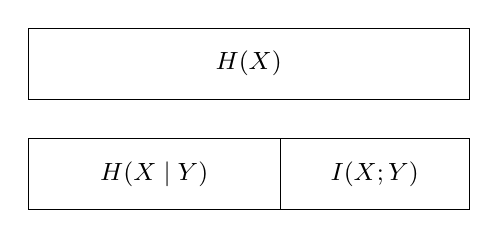
\begin{tikzpicture}[font=\small]
  % widths
  \def\hxgy{3.2}   % H(X|Y)
  \def\mi{2.4}     % I(X;Y)
  \def\H{0.9}      % box height
  \def\G{0.5}      % vertical gap
  \pgfmathsetmacro{\HX}{\hxgy+\mi}

  % bottom: H(X|Y) | I(X;Y)
  \draw (0,0) rectangle (\hxgy,\H);
  \node at (\hxgy/2,\H/2) {$H(X\mid Y)$};
  \draw (\hxgy,0) rectangle (\HX,\H);
  \node at (\hxgy+\mi/2,\H/2) {$I(X;Y)$};

  % top: H(X)
  \draw (0,\H+\G) rectangle (\HX,2*\H+\G);
  \node at (\HX/2,\H+\G+\H/2) {$H(X)$};
\end{tikzpicture}
\end{center}



\end{defn}

\section{Convexity and Jensen's Inequality}

In the following we give some definitions and theorems related to convex functions. For the most part, we will relegate the proofs to the textbook.  
\begin{defn}{Convexity  }{}
A real-valued function \(f(x)\) is said to be \textit{convex} over an interval \((a,b)\) if for every \( x_1,x_2 \in (a, b)\) and \(0\leq \lambda \leq 1\),  

\[
  f(\lambda x_1 + (1 -\lambda )x_2) \leq  \lambda f(x_1) + (1 -\lambda )f(x_2)
\]
A function \(f\) is said to be \textit{strictly } convex if equality only holds if \(\lambda = 0\) and \(\lambda = 1\). A function \(f\) is \textit{concave } if \(- f\) is convex.

\end{defn}


\begin{thrm}{}{}
If the function \(f\) has a second derivative that is nonnegative (positive) over an interval, the function is convex (strictly convex) over that interval. 


\end{thrm}


\begin{thrm}{Jensen's Inequality}{}
If \(X\) is a real-valued random variable and \(f(x)\) is a convex function, then
\[
  \mathbb{E} \left[ f(X) \right] \geq f \left( \mathbb{E} [X] \right). 
\]
It is important to note that the inequality flips if the function \(f\) is concave instead. 
\end{thrm}

\begin{thrm}{Properties of Mutual Information}{}
Recall the definition of mutual information:
\[
  I(X;Y) \coloneqq H(X)- H(X \mid Y) = H(Y) - H(Y \mid X) = H(X)+ H(Y)- H(X,Y) = I(Y;X). 
\]
Below we list some  properties of \(I(X;Y)\). 
\begin{enumerate}
  \item \(I(X;Y)\) is symmetric, this can be worked out by manipulating the definitions. 
  \item \(I(X;Y) \geq 0\) 
  \item \(I(X;Y) = 0 \iff X \text{ and } Y \text{ are independent }  \) 
\end{enumerate}
\end{thrm}

The figure below tries to illustrate the relationships between entropy and mutual information.


\begin{figure}[h]
  \centering
  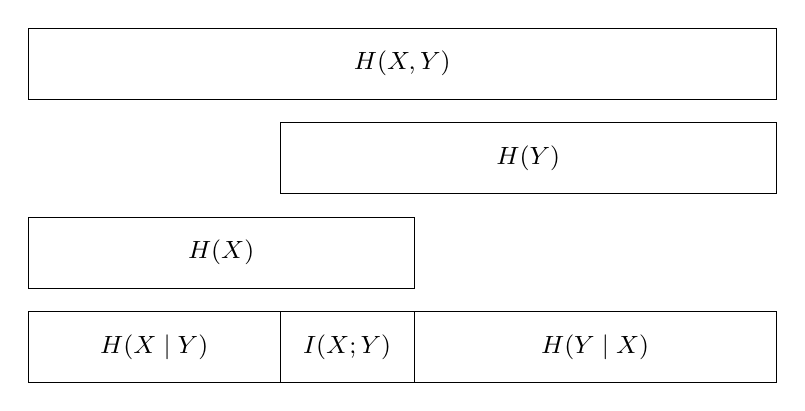
\begin{tikzpicture}[font=\small]
  % --- widths (cm): change to taste
  \def\hxgy{3.2}   % H(X|Y)
  \def\mi{1.7}     % I(X;Y)
  \def\hygx{4.6}   % H(Y|X)
  \def\H{0.9}      % box height
  \def\G{0.3}      % vertical gap

  \pgfmathsetmacro{\W}{\hxgy+\mi+\hygx} % total width
  \pgfmathsetmacro{\HX}{\hxgy+\mi}      % H(X) width
  \pgfmathsetmacro{\HY}{\mi+\hygx}      % H(Y) width

  %---------------------------------------
  % bottom row: H(X|Y) | I(X;Y) | H(Y|X)
  \draw (0,0) rectangle (\hxgy,\H);
  \draw (\hxgy,0) rectangle ({\hxgy+\mi},\H);
  \draw ({\hxgy+\mi},0) rectangle (\W,\H);

  % centers for bottom labels
  \pgfmathsetmacro{\cy}{\H/2}
  \pgfmathsetmacro{\cxA}{\hxgy/2}
  \pgfmathsetmacro{\cxMI}{\hxgy + \mi/2}
  \pgfmathsetmacro{\cxB}{\hxgy + \mi + \hygx/2}
  \node at (\cxA,\cy) {$H(X\mid Y)$};
  \node at (\cxMI,\cy) {$I(X;Y)$};
  \node at (\cxB,\cy) {$H(Y\mid X)$};

  %---------------------------------------
  % H(X) row (left)
  \draw (0,{\H+\G}) rectangle (\HX,{2*\H+\G});
  \pgfmathsetmacro{\cxHX}{\HX/2}
  \pgfmathsetmacro{\cyHX}{\H+\G + \H/2}
  \node at (\cxHX,\cyHX) {$H(X)$};

  % H(Y) row (right)
  \draw (\hxgy,{2*\H+2*\G}) rectangle (\W,{3*\H+2*\G});
  \pgfmathsetmacro{\cxHY}{\hxgy + (\W-\hxgy)/2}
  \pgfmathsetmacro{\cyHY}{2*\H+2*\G + \H/2}
  \node at (\cxHY,\cyHY) {$H(Y)$};

  %---------------------------------------
  % top row: H(X,Y)
  \draw (0,{3*\H+3*\G}) rectangle (\W,{4*\H+3*\G});
  \pgfmathsetmacro{\cxW}{\W/2}
  \pgfmathsetmacro{\cyHXY}{3*\H+3*\G + \H/2}
  \node at (\cxW,\cyHXY) {$H(X,Y)$};
  \end{tikzpicture}
  \caption{The big picture.}
  \label{fig:entropy-bars}
\end{figure}

\begin{thrm}{}{}

A useful tool to have is the following inequality:

\begin{align*}
    H(X) \leq \log |X|.
\end{align*}

  \tcbline
  \begin{proof} The following uses Jensen's inequality and the fact that the \(\log   \) function is concave,
\begin{align*}
    H(X) = \mathbb{E} \left[ \log \frac{1}{p(X)} \right] \leq \log \mathbb{E} \left[ \frac{1}{p(X)} \right] = \log \left\lvert X \right\rvert .
\end{align*}

\end{proof}
\end{thrm}
